\chapter{Social Interactions in AR}
\label{ch:annotation}

After studying the representation of social contacts (Chapter~\ref{ch:contacts}) and shared social data (Chapter~\ref{ch:data}), this chapter studies the interactions between social contacts with each other and other virtual objects. The interaction is represented by adding an AR tag or annotation on a shared medium to socially connect with other users.

The aim of this chapter is to answer the research question \ref{rq:data}: "How can wearable AR displays be used best for interacting with social contacts and shared social data?"
Annotation is one of the social interaction methods where users can add text or other information to be overlaid on top of a shared medium for the purpose of communicating ideas or thoughts between participants. In this chapter, we explore different media and options for sharing annotations with social contacts. AR annotations are useful for remote collaboration and shared experiences where context or descriptions of the conversation can be highlighted.  
The first section \ref{sec:video} addresses annotation of a live video stream. The second section \ref{sec:3D} studies annotation of a 3D environment using 3D sensors to detect the shared surrounding environment. The last section \ref{sec:pano} looks into panorama images as a medium and explores awareness and collaboration techniques. 

\section{Registration of AR Annotation on Social Video Sharing}
\label{sec:video}

AR annotation is an example of the interaction dimension on the Social AR Continuum. The registration of these annotations with respect to the user (viewer or sharer) can be represented in different level of detail (e.g., world-stabilised, body-stabilised and head-stabilised \cite{Billinghurst1998}) which can be mapped based on the social proximity. 

This section investigates an AR interface displaying comments directly on a live-streamed video. Our prototype allows remote spectators to perceive the streamed live video with different interfaces for displaying the comments, including an interface which puts AR annotation feedback directly on the shared video, and another interface that provides feedback in a separate window \cite{Nassani2016}. A user study was conducted to compare different ways of visualising comments and found that users prefer having comments directly in the AR view rather than in a separate list. This section discusses the implications of this research and directions for future work.

% Tobias: You did not really justify why you choose this specific visualisations/interfaces. You could state that it was inspired by YouTube or other media, but again, I think you need to justify your choice. Have there been other options, and why did you not choose them.

%  Tobias: You come directly from what the chapters do to your prototype. I would more appreciate if you integrate Figure 6.2 and use it to explain your envisioned scenario and context. From there, you can start to transition into the description of the prototype.

The vision of this work is to explore different user interfaces where users can add comments on a shared social video. Options considered based on existing video sharing platforms (e.g., YouTube\footnote{https://www.youtube.com/}, Vimeo\footnote{https://vimeo.com/}): (1) List, (2) Augmented Reality (AR), and (3) List + AR (see Figure \ref{fig:mgia16:conditions}).

\begin{figure}
  \includegraphics[width=\columnwidth]{images/61-video-mgia16/screenshots-enhanced-02}
  \caption{Overview of the investigated interfaces showing screenshots of the different interface conditions. (L): Comments displayed as a List on the side. (AR): Comments overlaid on the background video. (L+AR): Comments displayed both as a list on the right and as an overlay. }
  \label{fig:mgia16:conditions}
\end{figure}

Previous work has demonstrated live video sharing on a mobile platform and support for viewer feedback. However, there has been little evaluation of different methods for providing feedback. This section reports on investigations into different user interface (UI) options for viewing comments left by multiple users on a shared live video stream. Thus, the main contribution is investigating if comment placement on live video sharing improves the user experience. This work describes the prototype developed to explore this question.

\subsection{System Design}

In order to explore different ways to share AR comments from remote collaborators, a prototype was developed that enables a user to share a live video stream with others and receive comments from multiple users who are watching. Our system consists of a WebRTC\footnote{https://webrtc.org} application running on AppEngine\footnote{https://appengine.google.com/} on Google Cloud servers, which offers a fast peer-to-peer connection between devices. The advantage of the system being built on a web platform is that it can run on multiple hardware specifications, including desktop, hand-held, and wearable devices. Figure \ref{fig:mgia16:system} shows the overall design of the prototype system.

\begin{figure}[ht]
  \centering
  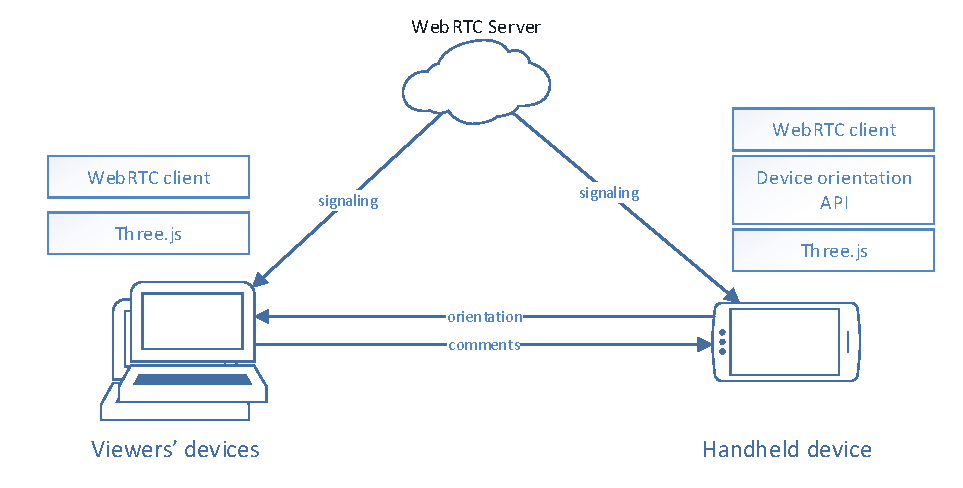
\includegraphics[width=\linewidth]{images/61-video-mgia16/system}
  \caption{System architecture of AR annotation on video streaming based on WebRTC}
    \label{fig:mgia16:system}
\end{figure}

The prototype was built as a fork from AppRTC\footnote{https://apprtc.appspot.com/} code base which hosts a website that enables people to start a video conferencing session on the web. The solution was built using an AppRTC base code was utilised to track device orientation by listening to the device sensors, and transferring the data to the receivers' devices via DataChannel. The AppRTC application is written in Python for the backend and Javascript for the front-end. It takes advantage of being hosted on AppSpot so that it complies with the WebRTC requirements for HTTPS. The AppRTC system allows users to communicate with each other over the Internet. The Three.js library\footnote{http://threejs.org/} was used. The AR visualization is implemented with two graphical layers (see Figure \ref{fig:mgia16:layers}). The background layer shows the video stream captured by the camera on the mobile device. On top of the background, comments are drawn on the front layer using orientation tracking information to show them in a body-stabilised manner. 

\begin{figure}[ht]
  \centering
  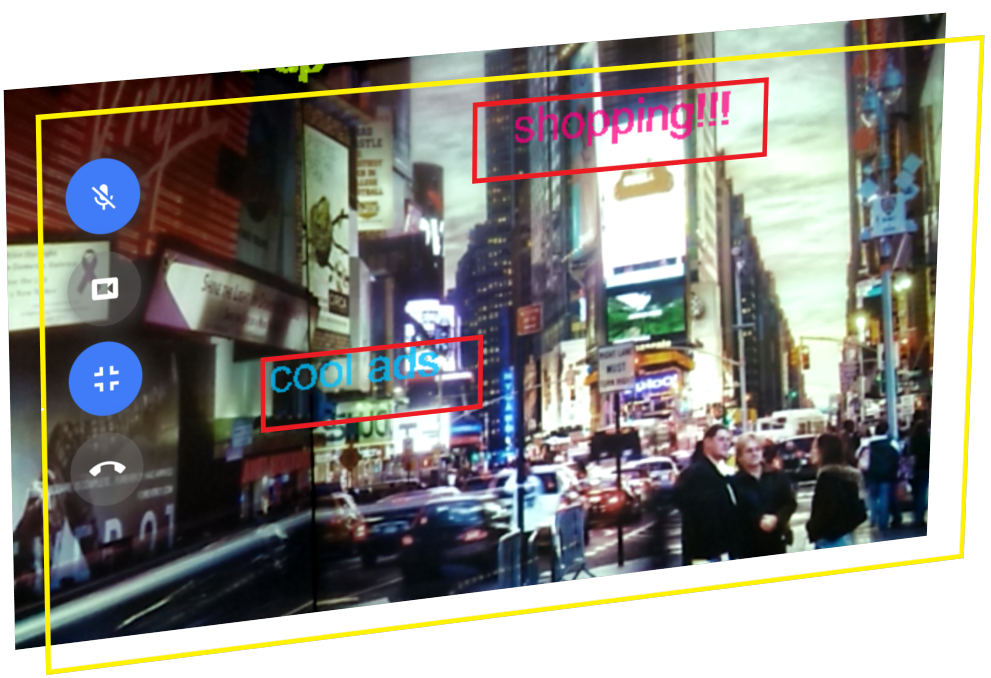
\includegraphics[width=0.8\linewidth]{images/61-video-mgia16/layers.png}
  \caption{UI of the system showing: 1) video layer (yellow) and 2) annotation layer (red)}
    \label{fig:mgia16:layers}
\end{figure}

\subsection{Implementation}

The application starts by turning on the back camera on the mobile device and asking the user to enter a "room number" to start the connection. Once this is entered, the application will enter "call mode", waiting for other participants to enter the same room number. Once the call is established, the mobile device will start streaming video and device orientation data to the viewing PC. 

Both users can send comments to each other by clicking on any part of the shared video. The system then calculates the 3D position of the comment in the AR space and waits for the comment text to be entered. Once the user enters the message, the text is displayed on both the sender's and receiver's screens. The motion data of the sender's device is also shared so that the receiver will see the comment appearing at the same place as the sender turns their device. 

Three different ways of showing comments on the live video stream are implemented (see Figure \ref{fig:mgia16:conditions} above). The first is a list view where the comments are listed on the side of the camera feed view. An AR view overlays comments on top of the video feed and rotated around the user based on phone orientation, so the comments appear fixed at the location on the video where they were first entered. Finally, an AR + list implementation combined the list view with the AR view. The next section reports on a user study exploring these three implementations.


\subsection{User Study}

A controlled within-subjects user experiment was conducted to test the different UIs for displaying comments, using the three approaches just explained. The experiment started with the participants giving consent and answering questions about demographic information. Then they went through a training session to get familiar with the application and the experimental procedures. The tasks during the training were designed to try to look around and read the comments appearing on the UI. A 180-degree panoramic image projected around the user on large screens was used to simulate different real spaces for the user (see Figure \ref{fig:mgia16:participant}). 

\begin{figure}[ht]
  \centering
  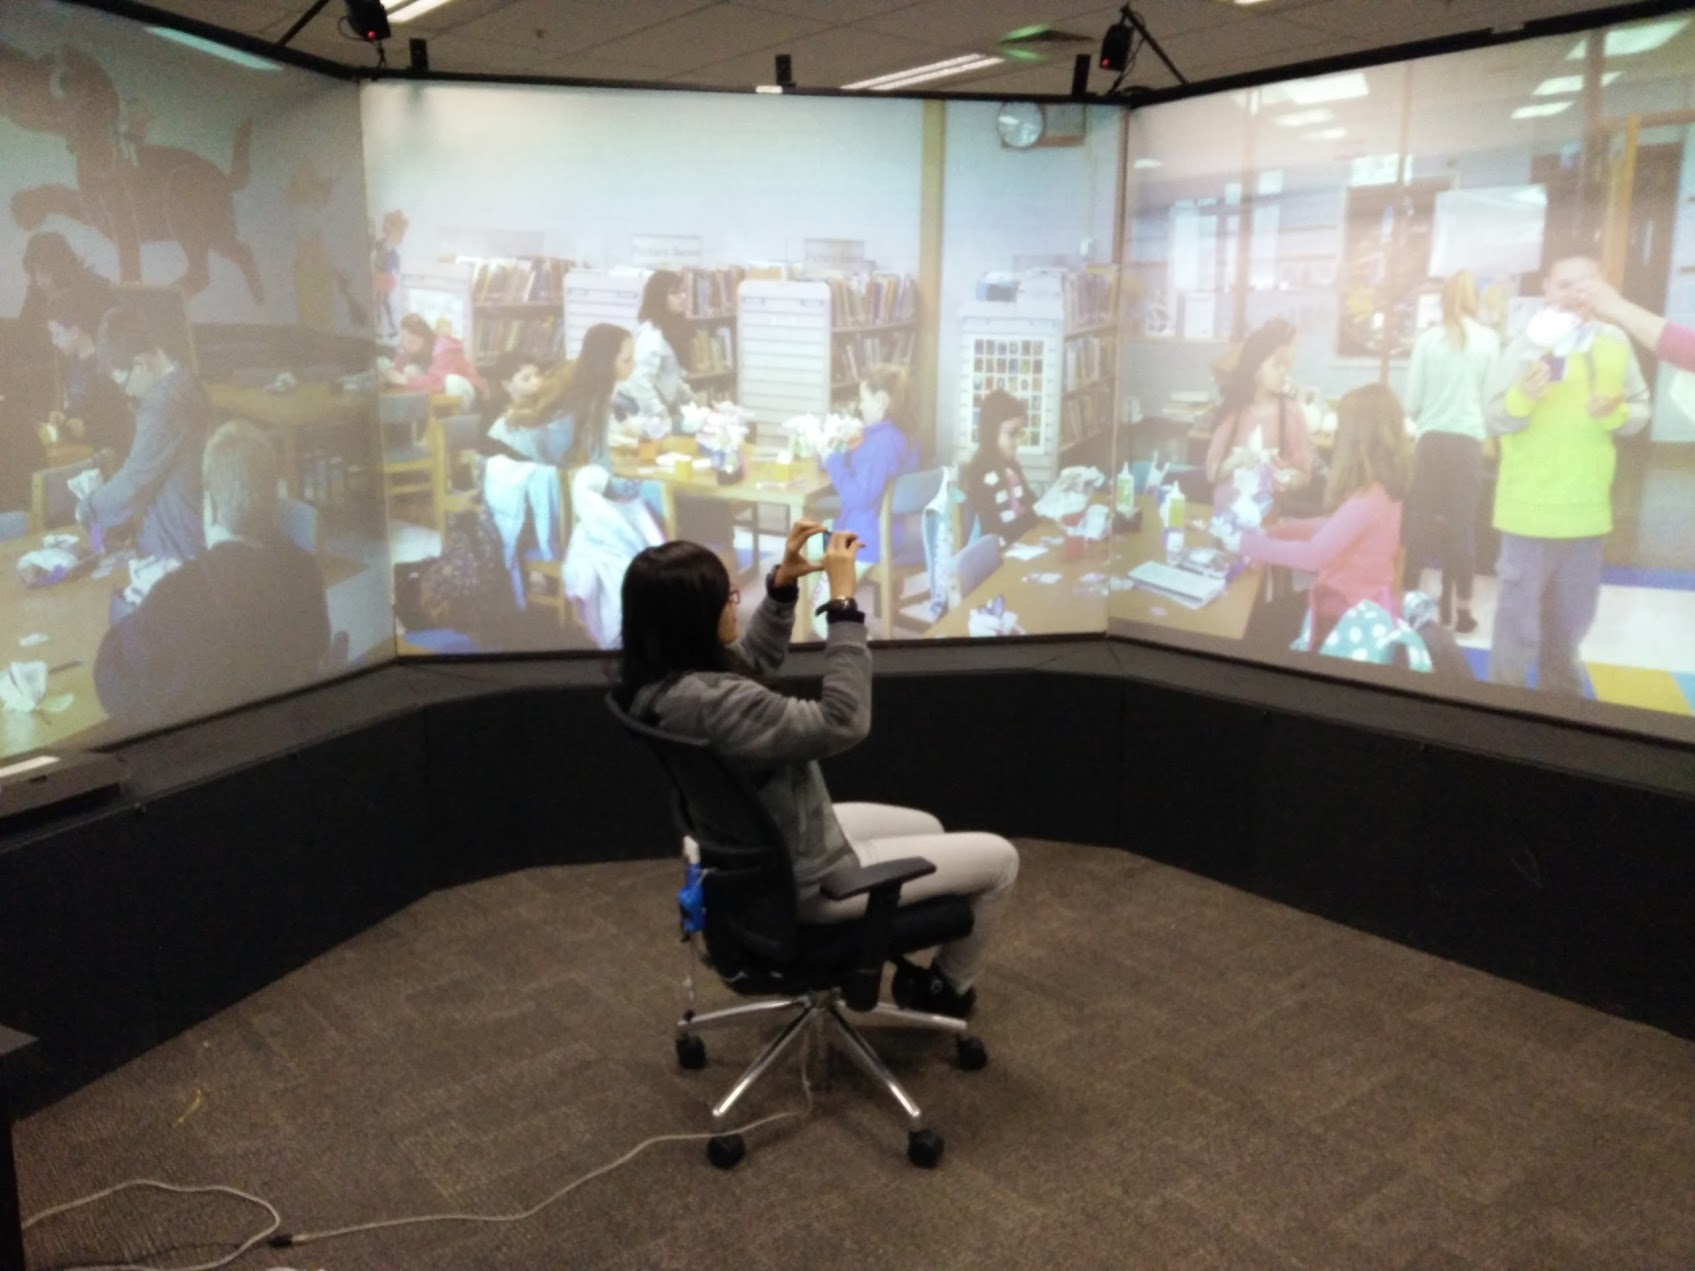
\includegraphics[width=0.45\linewidth]{images/61-video-mgia16/participant1}
  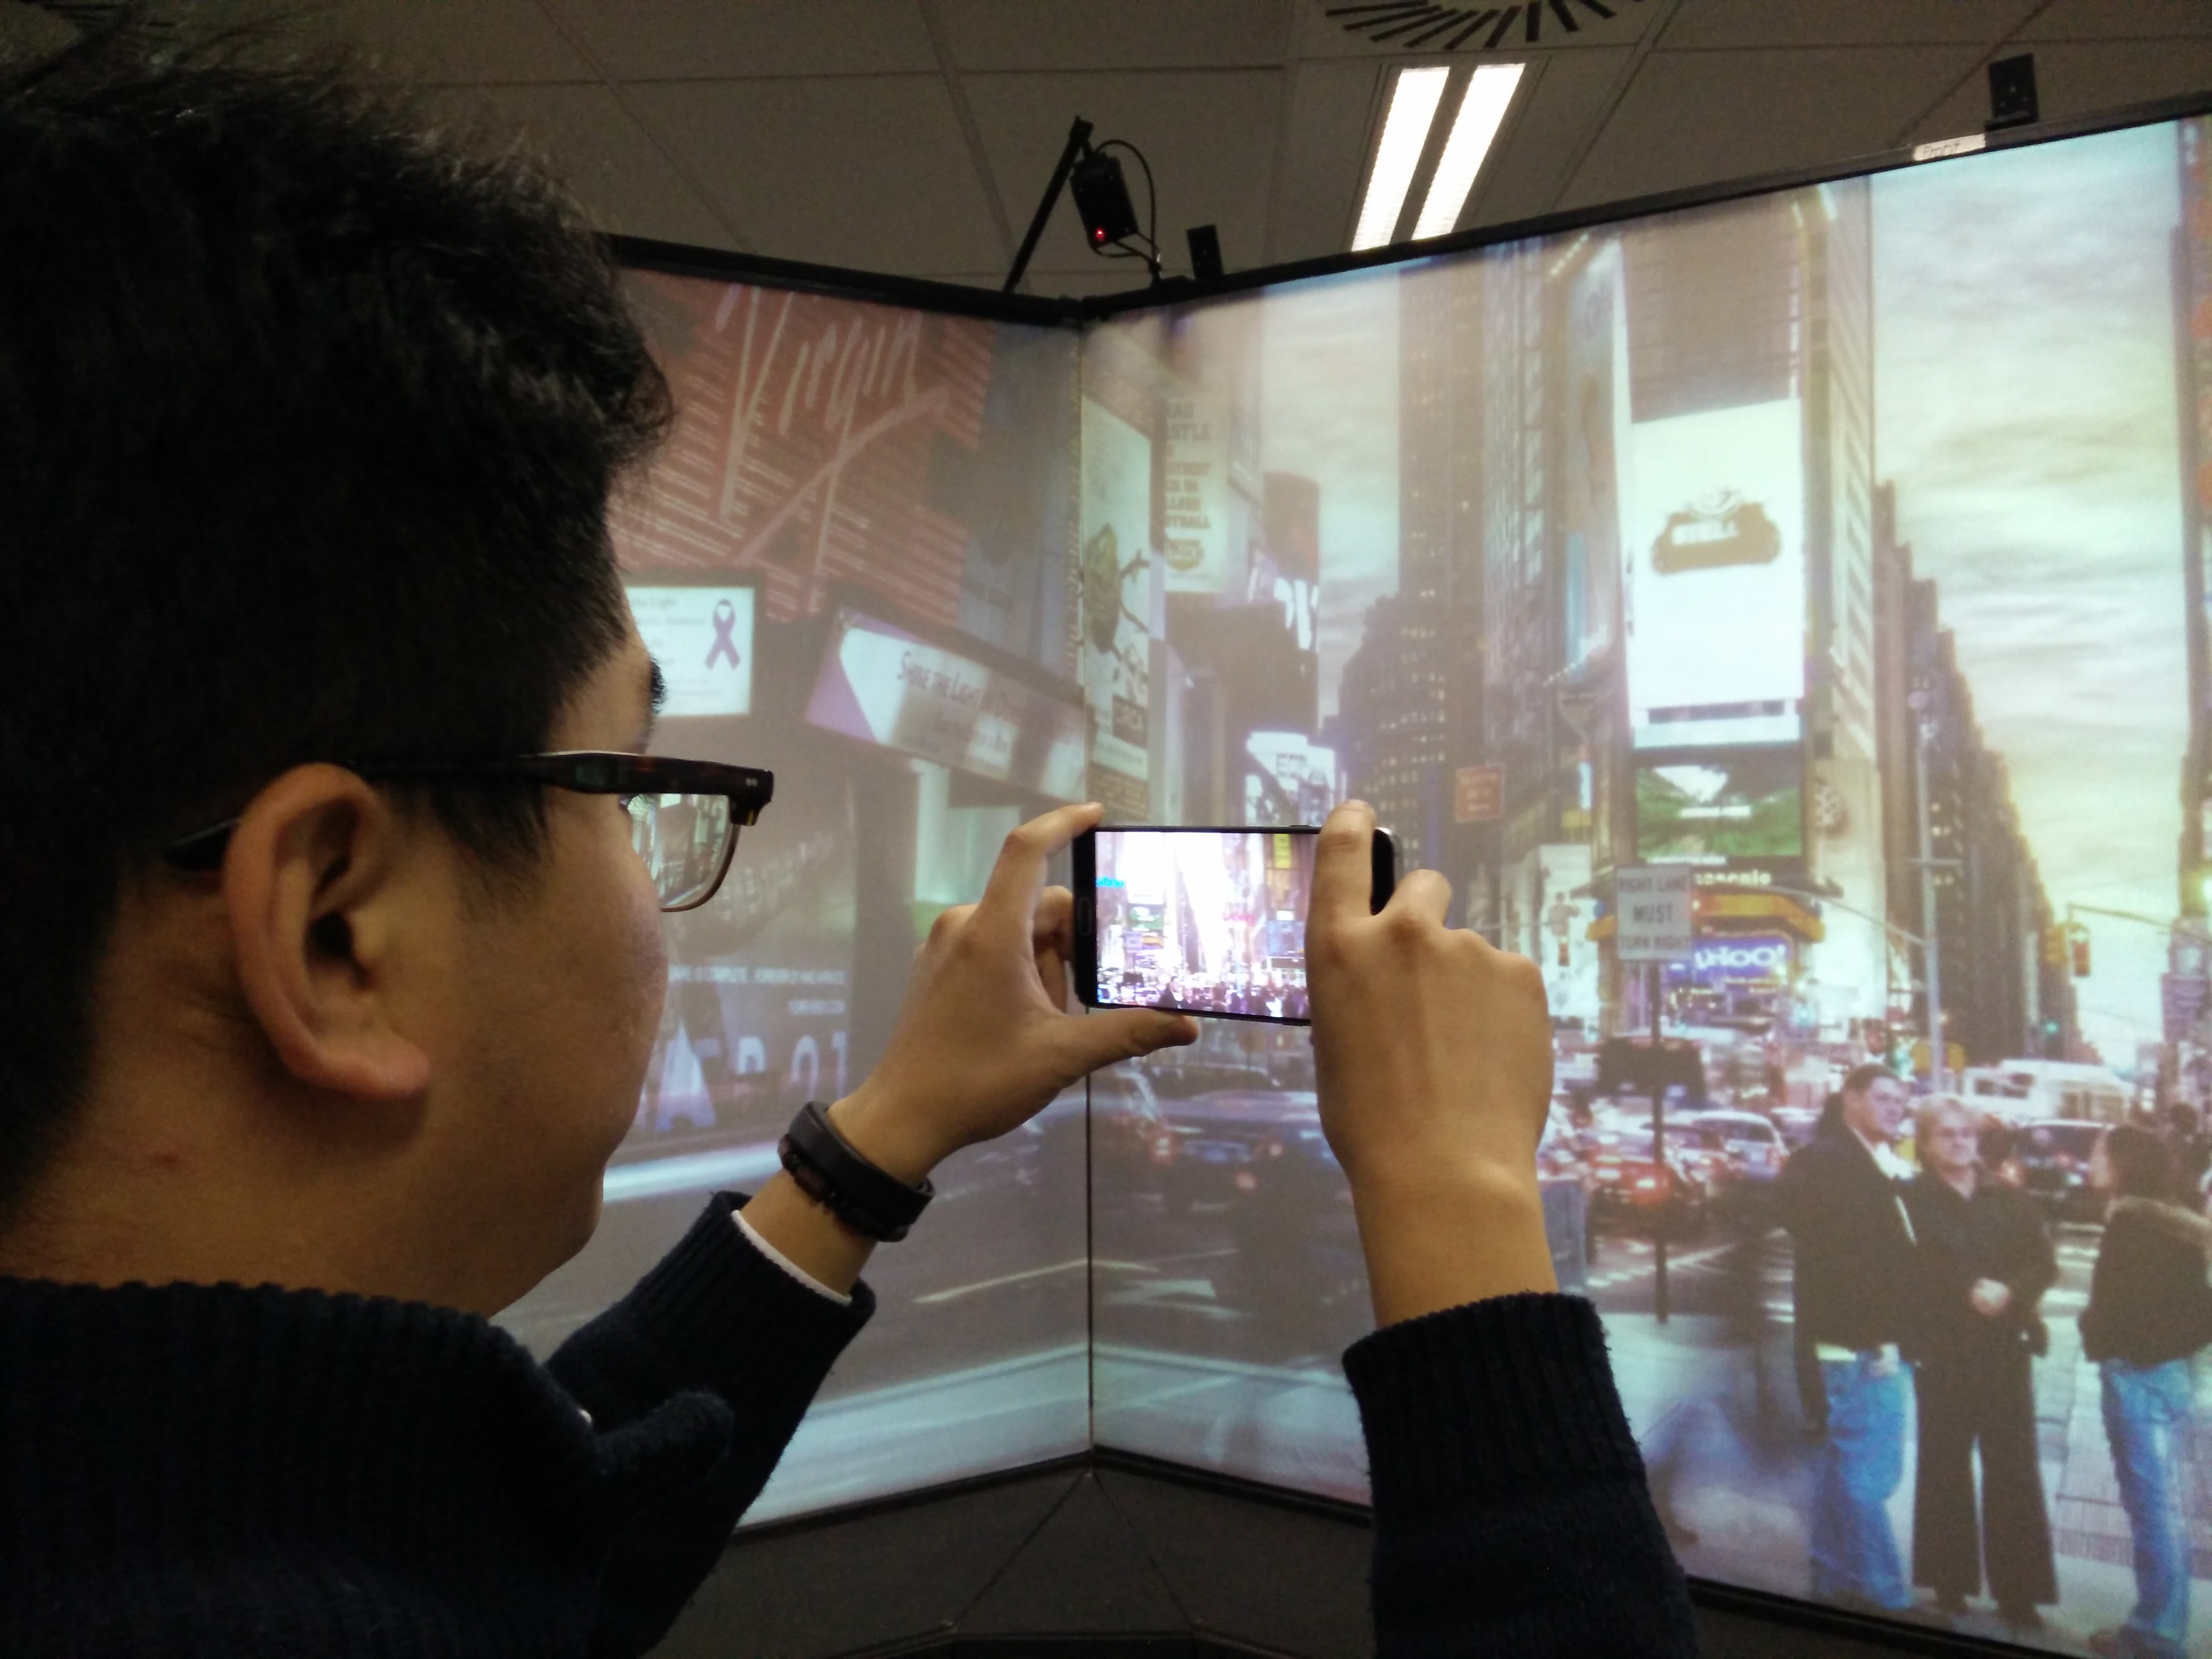
\includegraphics[width=0.45\linewidth]{images/61-video-mgia16/participant2}
  \caption{Participants during the experiment}
    \label{fig:mgia16:participant}
\end{figure}

Four different images were selected where the user might be interested in sharing their surroundings, varying in terms of indoors/outdoors and busy/quietness (see Figure \ref{fig:mgia16:backgrounds}). A different background was randomly assigned for each condition between subjects. 

\begin{figure}[ht]
  \centering
  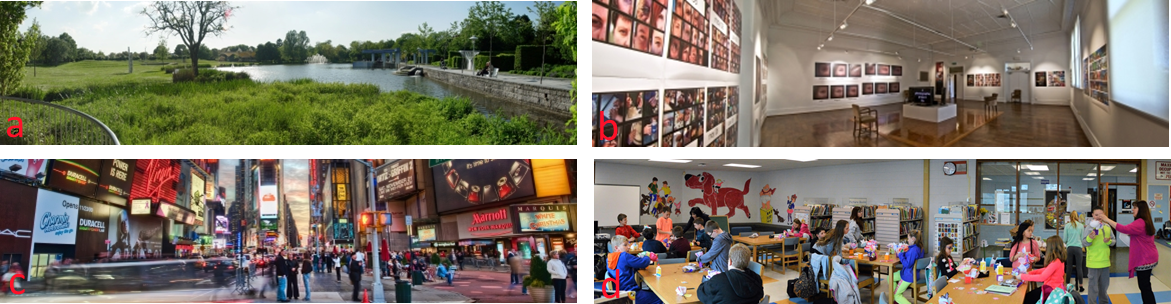
\includegraphics[width=\linewidth]{images/61-video-mgia16/backgrounds-legend.png}
  \caption{180-degree images used during the experiment. a) A park: outdoors and quiet, b) A museum: indoors and quiet, c) Intersection: outdoors and busy, d) A classroom: outdoors and busy.}
    \label{fig:mgia16:backgrounds}
\end{figure}

Each participant was asked to sit in the middle of the projection screens showing the background image, hold a smartphone, and aim its camera at the background to share it with remote users. The experimenter simulated multiple users sending comments on the shared video in a 'Wizard of Oz' style setup. There were six predefined comments (see Table \ref{table:mgia16:comment}) for each background. The predefined comments allowed for a controlled experiment (i.e., the same text at the same location) and reduced the need to have participants playing the role of the commenter. 

The comments appeared on the screen in three different styles depending on the experimental condition. The order of the conditions was counterbalanced using a balanced Latin square design. While watching the comments, the participant was asked to remember which part of the background each comment was talking about and who made a comment, which could be identified by the colour of the comment. There were up to four colours (commenters) in the experiment. The comments faded away one minute after being displayed, simulating the user receiving multiple comments while having limited time to read them all.

\begin{table}[h]
  \centering
  \caption{Social comments appeared on the 360 panoramic images during experiments}
  \label{table:mgia16:comment}
  \begin{tabular}{ |c|c|c|c| } 
\hline
    B1: Park    & B2: Museum  &   B3: Intersection    &  B4: Classroom\\
\hline
    nice place  &   interesting &  too many people & interesting \\
    picnic area &   beautiful   &  exciting  & busy \\
    play area   &   weird   &  shopping!!! & teacher \\
    nice lake   &   how much?    &  cool ads    & boring \\
    relaxing    &   confusing   &  people    & alone \\
    good for running    &   nice composition    &  traffic jam & what time is it\\\hline
  \end{tabular}
\end{table}

After completing a condition, participants were asked to place a printed version of each comment on a background image, at the correct location, and with the correct colour, testing their knowledge of where each comment appeared. The participants were also requested to answer a questionnaire on system usability \cite{brooke1996sus} and social presence \cite{Harms2004}. The social presence questions were slightly modified to fit the scenario being tested and only focused on one-way communication. Table \ref{table:social_questions} shows the social presence questions that were answered on a seven-level Likert-like scale rating (1: strongly disagree - 7: strongly agree). 

\begin{table}[h]
  \centering
  \caption{Social presence questionnaire. Negative questions marked with (-)}
  \label{table:social_questions}
  \begin{tabular}{ll}
    Q1 & Comments from others were clear to me.          \\
    Q2 & It was easy to understand comments from others. \\
    Q3 (-) & Understanding others' comments was difficult.  \\
    Q4 & I could tell how others felt by my video sharing.\\
    Q5 (-) & Others' emotions were not clear to me.\\
    Q6 & I could describe others' feelings accurately.
  \end{tabular}
\end{table}

% [do you want to show system usability questions as well?]

After finishing all three conditions, participants answered a post-experiment questionnaire that asked them to rank and compare all three conditions in terms of strengths and weaknesses. Finally, the experiment ended with a debriefing and the opportunity for participants to provide open-ended comments.

\subsection{Results}

Twenty participants (11 female, aged between 19 and 35 years old, Median=27.5, SD=4.55) were recruited to participate in the user study. Most (95\%) of them had experience with live video streaming a few times a week to a few times per month, and 80\% were familiar with AR applications. A Shapiro-Wilk test indicated that the data was not normally distributed. A non-parametric Friedman test was run for all the results with alpha=0.05, and post-hoc tests using Wilcoxon signed-rank tests with the Bonferroni correction ($alpha=0.017$).

The average SUS scores for each condition are shown in Figure \ref{fig:mgia16:questions_sus}. There was a statistically significant difference between the average SUS scores for each condition ($\chi^2(2)=9.658, p=0.008$). Post-hoc analysis showed significant differences between L and AR ($Z=-2.638, p=0.008$) and between L and L+AR ($Z=-2.559, p=0.010$). However, there was no statistically significant difference between AR and L+AR ($Z=-0.197, p=0.844$). This shows that the list condition on its own was considered considerably less usable than the other two conditions.

\begin{figure}[htb]
  \centering
  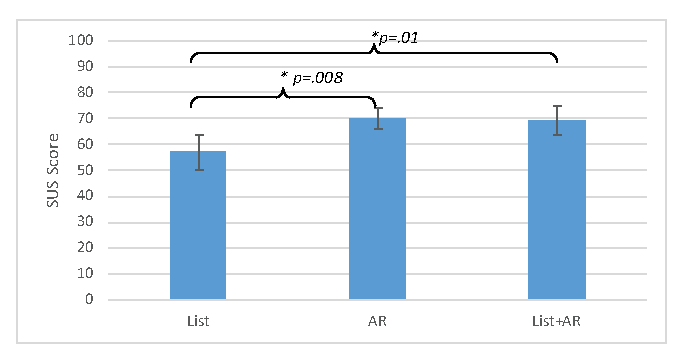
\includegraphics[width=0.8\linewidth]{images/61-video-mgia16/sus2.eps}
  \caption{SUS scores for each condition}
  \label{fig:mgia16:questions_sus}
\end{figure}

As for the social presence questions (see Figure \ref{fig:mgia16:social_presence}), the responses were inverted on the negative questions, Q3 and Q5, to allow all questions to be aggregated, combining the answers for both "perceived message understanding" and "affective understanding". There was a statistically significant difference in the perceived social presence ($\chi^2(2)=16.892, p<0.001$). Post-hoc analysis found there were significant differences between L and AR ($Z=-3.459, p=0.001$) and between L and L+AR ($Z=-3.311, p=0.001$) while there was no statistically significant difference between AR and L+AR ($Z=-0.427, p=0.670$).

% There was a statistically significant difference in the perceived social presence ($\chi^2(2)=16.892, p<0.001$). Post-hoc analysis found there were significant differences between L and AR ($Z=-3.459, p=0.001$) and between L and L+AR ($Z=-3.311, p=0.001$) while there was no statistically significant difference between AR and L+AR ($Z=-0.427, p=0.670$). 

% This shows that the list condition (L) was perceived as being less mutual understand and therefore creating less social presence, and that viewer comments in this condition were less clear.

% Why do you think there was a difference between AR and L+AR for the comment placement accuracy? It would be good to discuss this.

\begin{figure}[htb]
  \centering
  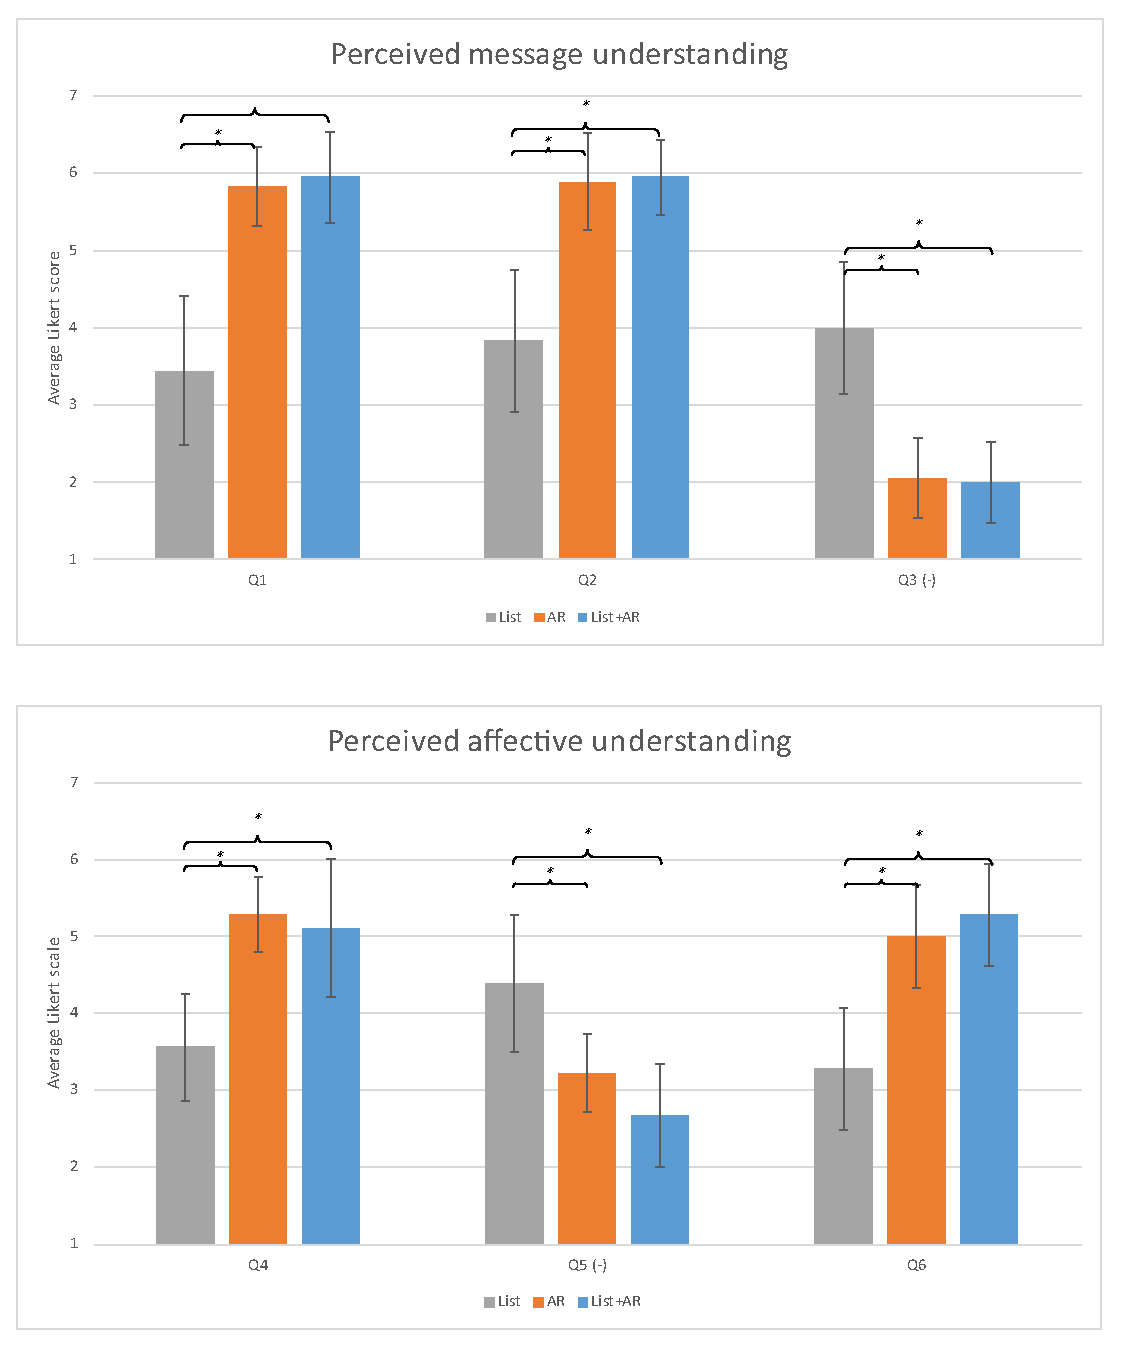
\includegraphics[width=.8\linewidth]{images/61-video-mgia16/social-presence.eps}
  \caption{Results for the social presence questions "perceived message understanding" and "perceived affective understanding". Whiskers indicate standard error. *=statistically significant difference}
    \label{fig:mgia16:social_presence}
\end{figure}

As for the ranking results (see Figure \ref{fig:mgia16:ranking}), the average of the answers (where 3=best, 1=worst) was calculated. The results show a statistically significant difference between conditions ($\chi^2(2)=9.100, p=0.011$). Post-hoc analysis showed a significance level set at $alpha$=0.017. There were significant differences between L and AR ($Z=-2.766, p=0.006$) and between L and L+AR ($Z=-2.502, p=0.012$). However, there was no statistically significant difference between AR and L+AR ($Z=-0.039, p=0.969$). This shows that the list condition (L) was ranked the worst out of the three conditions, and the two AR conditions were ranked the same.

\begin{figure}[htb]
  \centering
  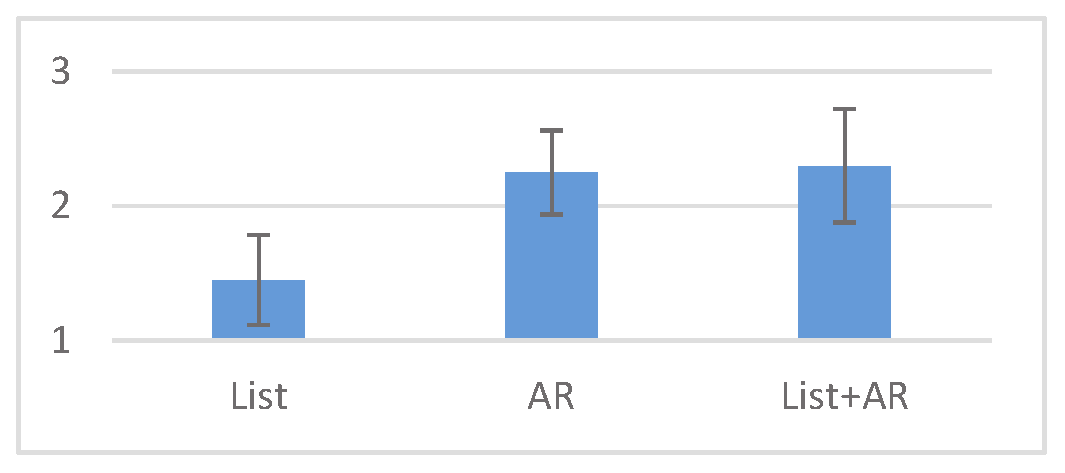
\includegraphics[width=.4\linewidth]{images/61-video-mgia16/ranking.eps}
  \caption{Results for condition ranking questions (3=best, 1=worst). Whiskers indicate standard error.}
    \label{fig:mgia16:ranking}
\end{figure}

For the task of matching the position and colour of the comments (see Figure \ref{fig:mgia16:questions_matching}) participants were asked to remember who wrote which comment (indicated by the colour of the comment) and the position of the comment (indicating which part of the scene the comment was about). The results show that there was a statistically significant difference ($\chi^2(2)=22.030, p<0.001$). Post-hoc analysis showed that there was no significant difference between the AR and L+AR conditions ($Z=-1.016, p=0.310$). However, there was a statistically significant difference between L and L+AR ($Z=-3.628, p<0.001$) and between L and AR conditions ($Z=-3.447, p=0.001$).

\begin{figure}[thb]
  \centering
  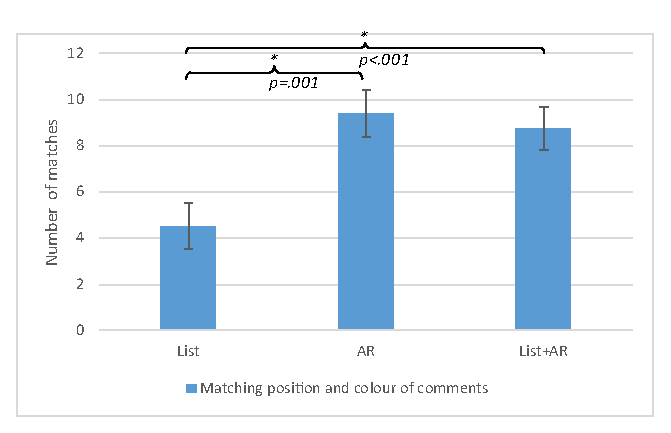
\includegraphics[width=.8\linewidth]{images/61-video-mgia16/matching-02.eps}
  \caption{Results for correctly matching comments with background and colour. Whiskers indicate standard error. *=statistically significant difference.}
    \label{fig:mgia16:questions_matching}
\end{figure}

Participants were asked open-ended questions to comment on their experience in terms of the strengths and the weaknesses of each condition. Approximately 80\% of feedback from the participants noted that in the list condition (L) it was more difficult to identify the area of the comments compared to the AR conditions. Eight participants (40\%) found it more challenging to remember the comment colours as a means to identify the person who sent the comment. 

In the AR and L+AR conditions, participants felt that the comments were contextual and relevant to the background. For example, \textit{"It is easier to remember comments on the video (AR) because the comments act as cues on the video you can directly see what the people are commenting on which I think makes me feel more connected to them"}. One of the strengths of the L+AR condition commented on included having an overview of the list of comments even if they are outside the current viewpoint of the user. 

However, users felt that comments in the L+AR condition could clutter the UI and partially block the background. One participant said \textit{"The screen just became too busy with comments that I do not have the time to actually sort out the comments and associate them on the video"}. Some suggested this could be resolved by making the comments not in the centre of view more transparent.
 
Participants were asked what they would like to improve. Most reported that they would like to use a head-mounted display to view comments in the AR mode.  It was also suggested to use a profile image instead of colours on comments to distinguish remote users.
 
Overall users felt that the AR and L+AR conditions were fun and cool to use, providing comments such as \textit{"It is pretty awesome. I love the experience, and I would really like to use this app with my social network."}.


\subsection{Discussion}

The user study results found that subjects preferred the conditions that contained an AR view, compared to showing comments only displayed in a list format. They thought these AR conditions were more usable than non-AR, provided a higher degree of social presence, and enabled them to remember the comment layout better. This is probably because the spatial association of comments increases the likelihood of the message being understood.
% Why do you think there was a difference between AR and L+AR for the comment placement accuracy? It would be good to discuss this

It was expected that one of the AR conditions (AR or L+AR) would have been more popular than the other; however, this was not the case. Some users preferred L+AR over the AR as the former provided an overall list of comments even if they were not visible in the current user viewpoint, making the user more aware of new comments without needing to look around to find them. Other users preferred the AR only condition, as the screen was less crowded. One solution to this might be hiding the comments on the list that are visible on the AR view, removing any duplication. Alternatively, a radar view could be used to show dots to represent comments. 

% It was learned that more about how to make live streaming a better experience for the user. 
Some users found the one-minute timeout for the comments fading away to be too fast. Associating the comments with colour to represent different users may not be the best option. An alternative approach would be to use an avatar or name of the person to identify the comment source. 

The study has a number of limitations that have to be addressed in the future. The experiment was conducted in a simulated environment rather than outdoors. A static background image was used to simplify the conditions. However, in real life, things will be moving in the background (e.g., people walking, cars passing by). In such scenarios, the comments in the AR condition may not stick to the moving objects. However, this could be solved by using image processing techniques to track objects that will allow the comment to be moved with them. Finally, all of the comments were generated by an experimenter and were fixed, rather than coming from real people who could write whatever they liked.    

\subsection{Conclusions}

This section investigated AR annotations for social live video streaming. The work included conducting a user study testing three variations of the interface for showing comments: 1) a List view, 2) an AR view and 3) a combined List + AR view. Participants felt that the AR and the List + AR conditions were significantly better than the List condition in terms of system usability and social presence. The following sections investigate the higher level of fidelity in AR annotations using 3D sensors and on panoramic images. 
\pagebreak
\section{AR Annotation using 3D sensors}
\label{sec:3D}

A second example of the interaction dimension of the Social AR Continuum is in interaction with 3D depth data. The AR annotation can be placed in a 2D plane (lower fidelity) or on a 3D depth registration (higher fidelity), which then can be mapped into social proximity. 

This section describes a wearable system that allows people to place and interact with 3D AR annotations placed around them (\cite{Nassani2015a, Nassani2015}, Figure \ref{fig:mgia15:teaser}). It uses two wearable technologies: a head-worn wearable computer (Google Glass\footnote{https://en.wikipedia.org/wiki/Google\_Glass}) and a chest-worn depth sensor (Google Tango \footnote{https://en.wikipedia.org/wiki/Tango\_(platform)}). Google Glass is used to generate and display virtual information to the user, while the Tango is used to provide robust indoor position tracking for the Glass. The Tango enables spatial awareness of the surrounding world using various motion sensors including 3D depth sensing, an accelerometer and a motion-tracking camera. Using these systems together allows users to create an AR annotation via voice input and then register this annotation to a physical object or position in 3D space as an augmented annotation. This work describes the design and implementation of the system, user feedback, research implications, and directions for future work.  

\begin{figure}[ht]
  \centering
  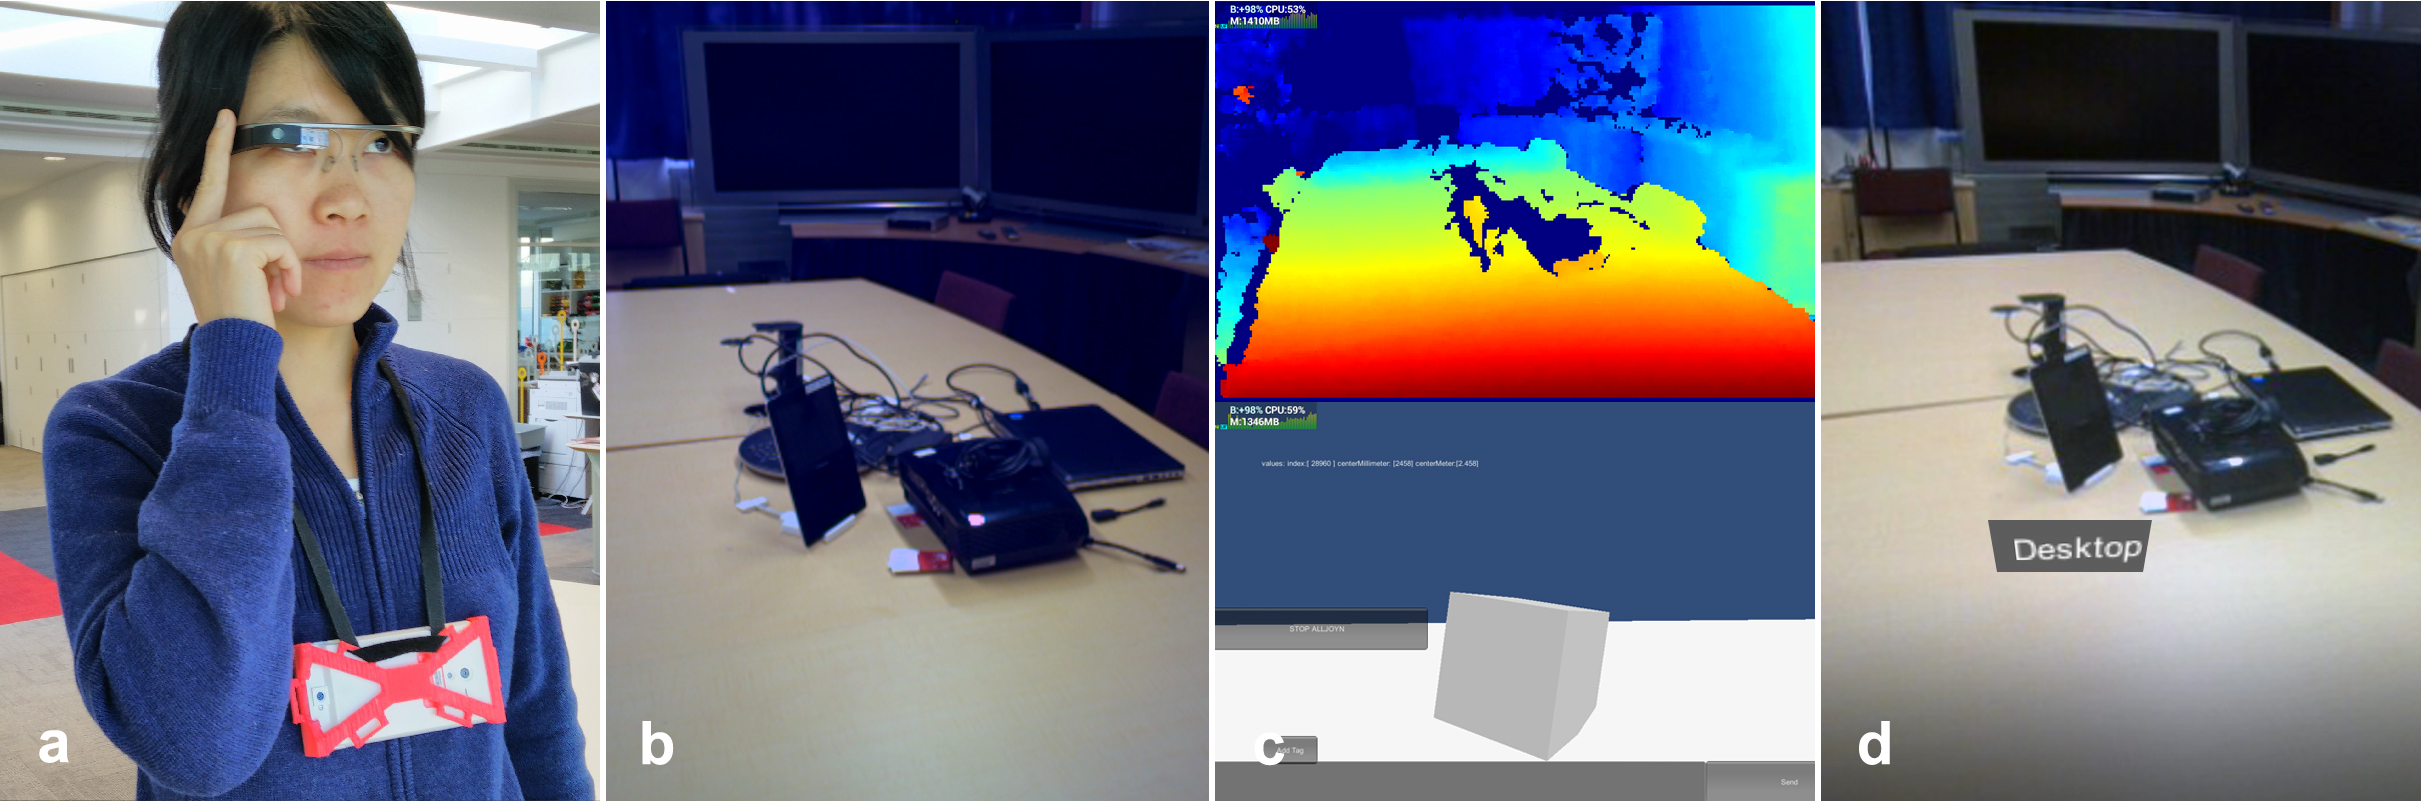
\includegraphics[width=\linewidth]{images/62-3d-mgia15/sampleteaser-01.jpg}
  \caption{AR annotation application scenario. (a) The setup; (b) A sample indoor environment; (c) The depth data from the Tango sensors; (d) The AR view through the Glass display.}
  \label{fig:mgia15:teaser}
\end{figure}

This system combines multiple wearable technologies through a wireless network. The system is small and light enough to be comfortably worn, allowing for mobility in the physical world, and being available for annotation not only on 2D surfaces also in 3D space. For example, if the user walks closer to or away from the AR annotation (e.g., 3D text or models), it will appear larger or smaller according to the changes in the perspective view. The system combines Google Glass and Google Tango together to provide a compelling wearable AR experience. Google Tango is a self-contained hand-held device that uses a motion-tracking camera, 3D depth sensing, a nine-axis accelerometer, gyroscope and compass sensors. It has a rear-facing 4MP RGB/infrared camera, a 180-degree field-of-view fisheye rear-facing camera, a 120-degree field-of-view front-facing camera, and a 320 x 180 depth sensor. In contrast, Google Glass has no depth-sensing capability but combines computing and display in a highly compact form factor. 

% Connecting the two devices enables us to prototype future wearable AR interfaces such as what might be possible with Microsoft Hololens\footnote{https://www.microsoft.com/microsoft-hololens/en-us} or other devices.


\subsection{System Design}

The main application scenario for our prototype system is around sharing messages through creating and viewing location-based AR annotations registered in a small scale physical environment. The user wearing the system walks into a room and then places AR annotations at various places or on objects offline (asynchronously) so that the AR annotation can be viewed later by the same user or by a different user. The AR annotation content is created by using voice input and placed where the user is looking. The distance between the AR annotation and the user is between 0.5 to 4 meters (according to Google Tango depth camera specifications) The AR annotations can be meaningful for users, for example, reminding them of something interesting in this space, or sharing the message with other users as a collaborative tool. The system should work in an arbitrary unprepared indoor environment where no previous knowledge about the space is required. 

Traditionally AR annotation tracking uses two different approaches at different ends of the technology spectrum (see Figure~\ref{fig:mgia15:spectrum}) based on the level of detailed information required. At one end, there is GPS location-based tracking that can be implemented in a light-weight HMD such as Glass. On the other end, 3D depth-sensing cameras incorporated into a hand-held device (HHD) are capable of indoor tracking and localisation. The aim of this system is to combine the benefits of a light-weight HMD with self-contained mobile 3D depth tracking, offering not only the outdoor GPS based tracking but also vision-based indoor tracking for AR annotation applications. 

\begin{figure}[ht]
  \centering
  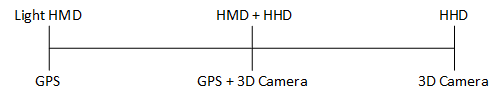
\includegraphics[width=0.8\linewidth]{images/62-3d-mgia15/tango_paper_continuum.png}
  \caption{The spectrum of AR annotation tracking. A head-mounted display with GPS is ideal for outdoor tracking. Hand-held devices (3D camera) can be used for indoor tracking. Glass+Tango enables indoor AR annotation tracking on a light HMD.}
  \label{fig:mgia15:spectrum}
\end{figure}

\subsection{Implementation}

The system consists of two wearable devices, a Google Glass HMD and a Google Tango chest-mounted 3D depth and sensor (see Figure~\ref{fig:mgia15:framework}). The two devices communicate with each other wirelessly. The Tango extends Glass' sensing ability by sharing the location and pose of the user as well as the annotated target position in the real world. The Glass dynamically overlays an AR annotation based on the spatial information received from the Tango, and the background of the Glass display is set to black to act as an optical see-through display (see Figure~\ref{fig:mgia15:ui}). A white square is displayed on the Glass screen to indicate the centre point at which the tango depth camera is facing. The user can initiate the wireless connection by using a three-finger touch gesture on the Glass touchpad, and the AllJoyn\footnote{https://en.wikipedia.org/wiki/AllJoyn} library is used for networking.

\begin{figure}[ht]
  \centering
  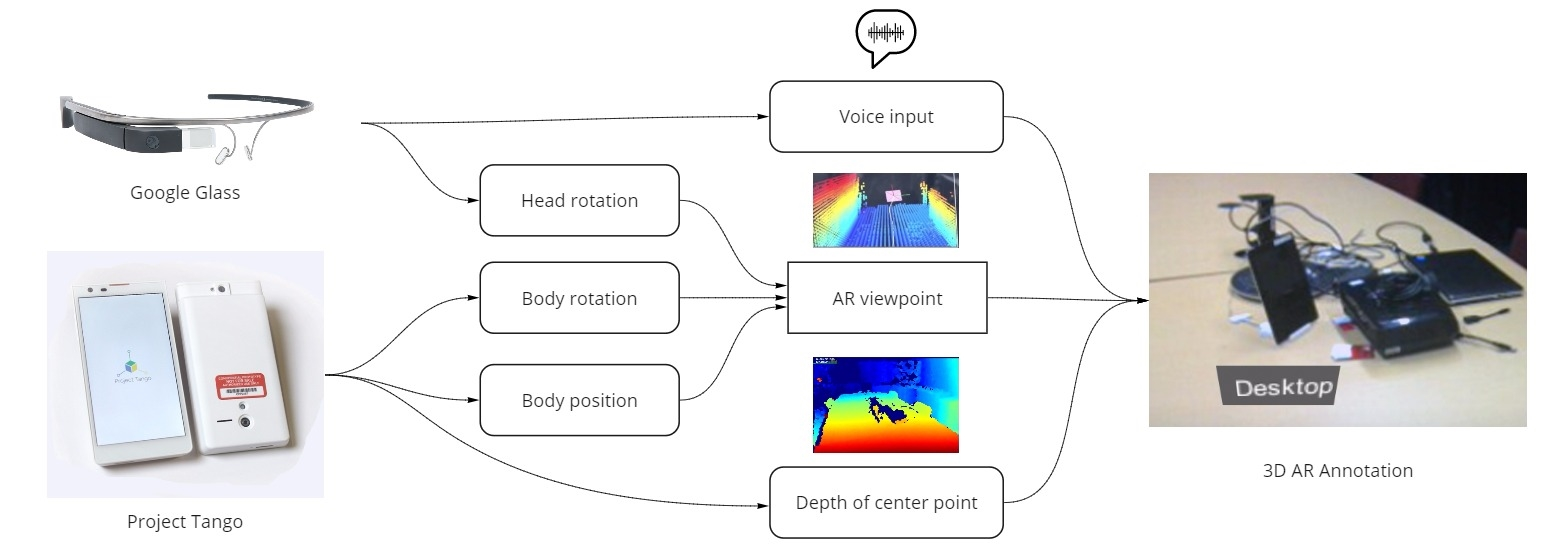
\includegraphics[width=\linewidth]{images/62-3d-mgia15/mgia2015-system.jpg}
  \caption{System workflow of AR Annotation using 3D sensors. Google Glass detects user voice input for the annotation text content. The AR viewpoint is calculated based on the head rotation from Google Glass, body rotation and position from Google Tango. Google Tango also provides the depth (z-axis) for where to place the annotation on top of the real world.}
  \label{fig:mgia15:framework}
\end{figure}

Once the system starts on the Tango, it creates a reference coordinate of the surrounding environment. When the user moves, the motion sensor on the Tango will detect the body position and rotation from the reference origin, both of which are then wirelessly transmitted to the Glass. Combing the head rotation detected by the sensors on the Glass, the AR Viewpoint position can be calculated. The position of the AR viewpoint is calculated by adding a measured distance in height from Tango's position to adjust for the height difference between the Glass and Tango. The orientation of the AR viewpoint mainly depends on the body's rotation but will be adjusted with the head and body pose difference, if the user turns their head towards a different direction from their chest. 

A speech recognition service is running in the background on the Glass to detect the users' voice input and convert it into a short-word text. The text will appear on the upper-left corner of the display for the user's confirmation (see Figure~\ref{fig:mgia15:ui}). The upper-left corner shows the last words captured via the voice recognition service, and a white square indicates the centre position of Tango's RGB depth frame. The text in the middle of the display "Cup" is an AR annotation overlaid on top of a physical cup. This function is implemented as an Android service that utilises the Google API for speech recognition\footnote{https://developers.google.com/glass/develop/gdk/voice} and so requires an internet connection. Once the user is satisfied with the recognised text, they can tap on the Glass touchpad while looking where they wish to add the AR annotation by using the white square in the display. The Glass sends a request to Tango to identify the location of the AR annotation in 3D space.

\begin{figure}
  \centering
  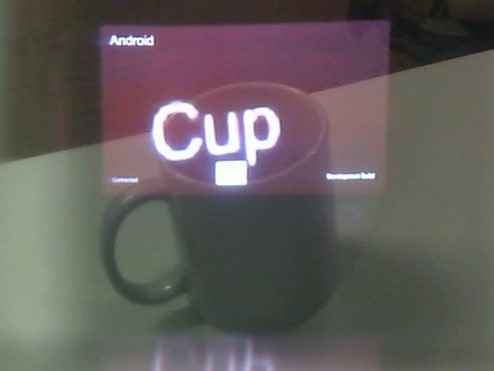
\includegraphics[width=0.6\linewidth]{images/62-3d-mgia15/WIN_20150614_204531_2.jpg}
  \caption{View through Glass display of a cup overlaid with an AR annotation.}
  \label{fig:mgia15:ui}
\end{figure}

Combining the AR viewpoint and the recognised text, the target position could be converted (the centre point of the depth image indicated by the white square) to the global position relative to the origin. The Tango returns the global position of the AR annotation to the Glass. This information is used to construct an AR annotation with the speech recognised text that is overlaid on the top of the Glass camera view.

\subsection{User Study}

A user study was conducted (see Figure~\ref{fig:mgia15:scenario}) with ten participants, four female, six male, ranging in age between 23 to 33 years old ($SD= 4.35$). The main focus of the study was to measure the usefulness of the proposed system. Participants were asked to create three different AR annotations for three different objects inside the room, with voice input, and then to walk around to observe how well the AR annotation was placed at the selected location. Participants had the freedom to assign a text using voice input to an object they wished in the test. The experimenter explained the task before the experiment and gave examples of target objects and names to use for voice input. All participants completed the task within five minutes. 

\begin{figure}
  \centering
  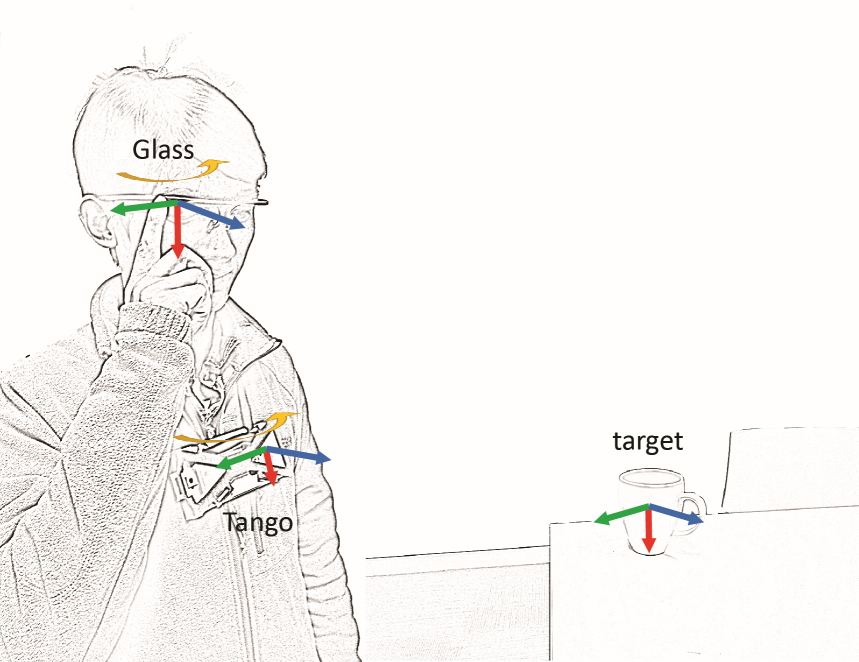
\includegraphics[width=0.6\linewidth]{images/62-3d-mgia15/axis_lo_small.jpg}
  \caption{User study scenario}
  \label{fig:mgia15:scenario}
\end{figure}

Qualitative feedback about the system was collected from participants, including how they would describe their experience using our system, what they liked and disliked. The same set of questions (Table \ref{table:mgia15:questions}) were asked in four categories: (C1) Using the voice commands to create an AR annotation, (C2) Tap on glass touch panel to attach the AR annotation, (C3)  Walk around to find an AR annotation stuck to the original position, (C4) Overall AR annotation experience.

\begin{table}
  \centering
    \caption{Survey questions}
    \label{table:mgia15:questions}
    \begin{tabular}{r l}
    \hline
    Q1 & I found it easy to use \\ \hline
    Q2 & I found it natural to use \\ \hline
    Q3 & I found it physically challenging \\ \hline
    Q4 & I found it mentally challenging \\ \hline
    Q5 & I found it useful \\ \hline
    \end{tabular}
\end{table}

\subsection{Results}

The answers were captured on a Likert scale of 1 to 7 in which 1 = "strongly disagree", and 7 = "strongly agree". The One-sample Wilcoxon Signed-Rank test was used on the results to measure significance. Based on the results, the results found that participants rated significantly higher than neutral (4) on Q3 ($p=0.01, 0.009, 0.007, 0.041$) and Q4 ($p=0.014, 0.009, 0.007, 0.01$) for all categories (C1, C2, C3, C4). Q2 ($p=0.033$) and Q5 ($p=0.015$) were rated significantly higher for category (C3). Q1 for C4 was rated significantly higher ($p=0.014$) (see Figure~\ref{survey_results}). The results for other tasks were rated less significant than neutral level (4). Participants rated the task of walking around the environment as useful with an average score of 5.2 out of 7, as well as being not mentally challenging with an average score of 2 out of 7. This highlights the usefulness of the system in assigning AR annotations and recognising them when they appear on their display while walking around the environment. 

\begin{figure}
  \centering
  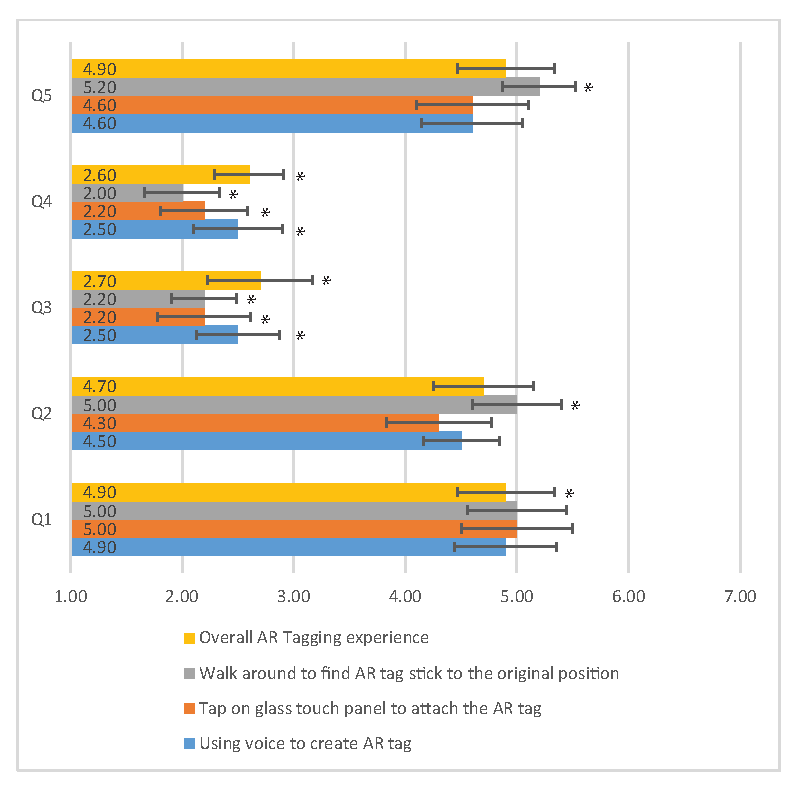
\includegraphics[width=.8\linewidth]{images/62-3d-mgia15/user_study_results2.eps}
  \caption{Average results of survey questions. Bars indicate standard error. *=statistically significant}
    \label{survey_results}
\end{figure}

In addition to the survey, participants were asked open-ended questions to comment on the system usability. A total of 3 out of 10 participants mentioned that they would use this system for virtual sticky notes, and they also provided some positive feedback such as "\textit{the system could be useful for finding a meeting room or a colleague's desk in an open plan area}". There were also a few suggestions for improving the system, such as "allow the user to manually adjust the location of the AR annotation" or "integrate with eye-tracking to assist placing the AR annotation within the field of view". Participants appreciated the concept of wirelessly connecting depth camera to a wearable HMD to enable the 3D spatial tracking.    

\subsection{Discussion}

While our prototype system demonstrates the concept of harmonising the use of multiple wearable devices for AR visualisation, there are a few limitations in the current implementation of the system. It was observed that some users had difficulties with voice input as they were not native English speakers, which made the participants use several attempts before the intended word was correctly recognised.  

The current system tracks the 3D environment relative to the starting position, which requires users to start the system at the same position and orientation in each test trail to keep the annotation in place between uses for sharing. This could be overcome in the future by storing the reconstructed 3D map of the environment and reusing it instead of generating it from scratch every time. 

% \subsection{Future Application Scenarios}
Many implementation scenarios could benefit from combining a light-weight HMD with a chest-worn 3D depth camera, such as 1) Navigation, 2) Remote collaboration and 3) Social sharing. This section describes each of these in more detail.

Navigation is a scenario where this system can be useful. The user could navigate in an outdoor environment using GPS on Glass or similar smart glass display. Google Glass, being an unobtrusive HMD, allows for hands-free navigation. However, when the user enters a building, the GPS stops working, and the system switches to indoor navigation using the 3D depth camera of the Google Tango device. Combining two devices enables a seamless transition during a navigation experience. For example, a person could be shopping to find a particular item and use outdoor GPS tracking to guide them to the store. Once inside the store, the Tango depth-sensing hardware can help with navigating to find a particular product on the shelf.

Remote collaboration is another scenario where this application could be useful. A local user could transmit reconstructed 3D geometry of the environment using the Tango device to the remote user. The remote user will then have a more detailed view of the environment compared to 2D sharing such as with a video stream. With the 3D geometry of the environment, the remote user can view the scene from different angles which helps provide a better understanding of the surroundings of the local user. Placing AR annotations in a 3D environment helps maintain the location of the AR annotation especially when the viewing perspective is changed to the point from when it was originally recorded

Additional use of the system could be in a social sharing experience where multiple users of the system could collaborate to add, edit and manipulate AR annotations in the shared environment. Multiple users wearing depth sensors could see the same annotation while they are face-to-face or if they are remote, they can see a live stream from the local user with the AR annotation. Also for asynchronous collaboration, user A can add an annotation to a physical object/location, then user B can come in later (when user A has left) and view and interact with the AR annotation.

The system described in this section was designed and implemented in 2014. In 2019, similar capabilities can be found in a self-contained HMD unit such as HoloLens or Magic Leap. If similar project objective, again today you could do this on the MagicLeap display with no additional hardware.


\subsection{Conclusions}

This section presented a wearable AR system combining tracking technologies to provide a compelling indoor AR experience for spatial annotation applications, especially in asynchronous collaboration scenarios where the users of the system are not required to be online at the same time. By wearing the system, users can create AR annotations with text content generated by voice input, and place them where they are looking. The AR annotation can be visualised in place as a reminder for the users.  


\pagebreak
\section{Social Panoramas Using Wearable Computers}
\label{sec:pano}

A third example of annotation as interaction dimension on the Social AR Continuum is an annotation on 360-degree panoramic images. The level of annotation can be described as drawing or adding text, which then can be mapped into social proximity. This section discusses using panorama images to share social experiences. In particular, it explores awareness and annotation cues between users sharing a social experience through a shared panoramic image.

This work describes the concept of Social Panoramas that combine panorama images, Mixed Reality, and wearable computers to support remote collaboration \cite{Reichherzer2014, Billinghurst2014} (Figure \ref{fig:ismar14:concept}). A prototype was developed that allows panorama images to be explored in real-time between a Google Glass user and a remote tablet user. This uses a variety of cues for supporting awareness and enabling pointing and drawing. A user study was conducted to explore if these cues can increase Social Presence. The results suggest that increased interaction does not increase Social Presence, but tools with higher perceived usability show an improved sense of Presence.

\begin{figure}
    \centering
    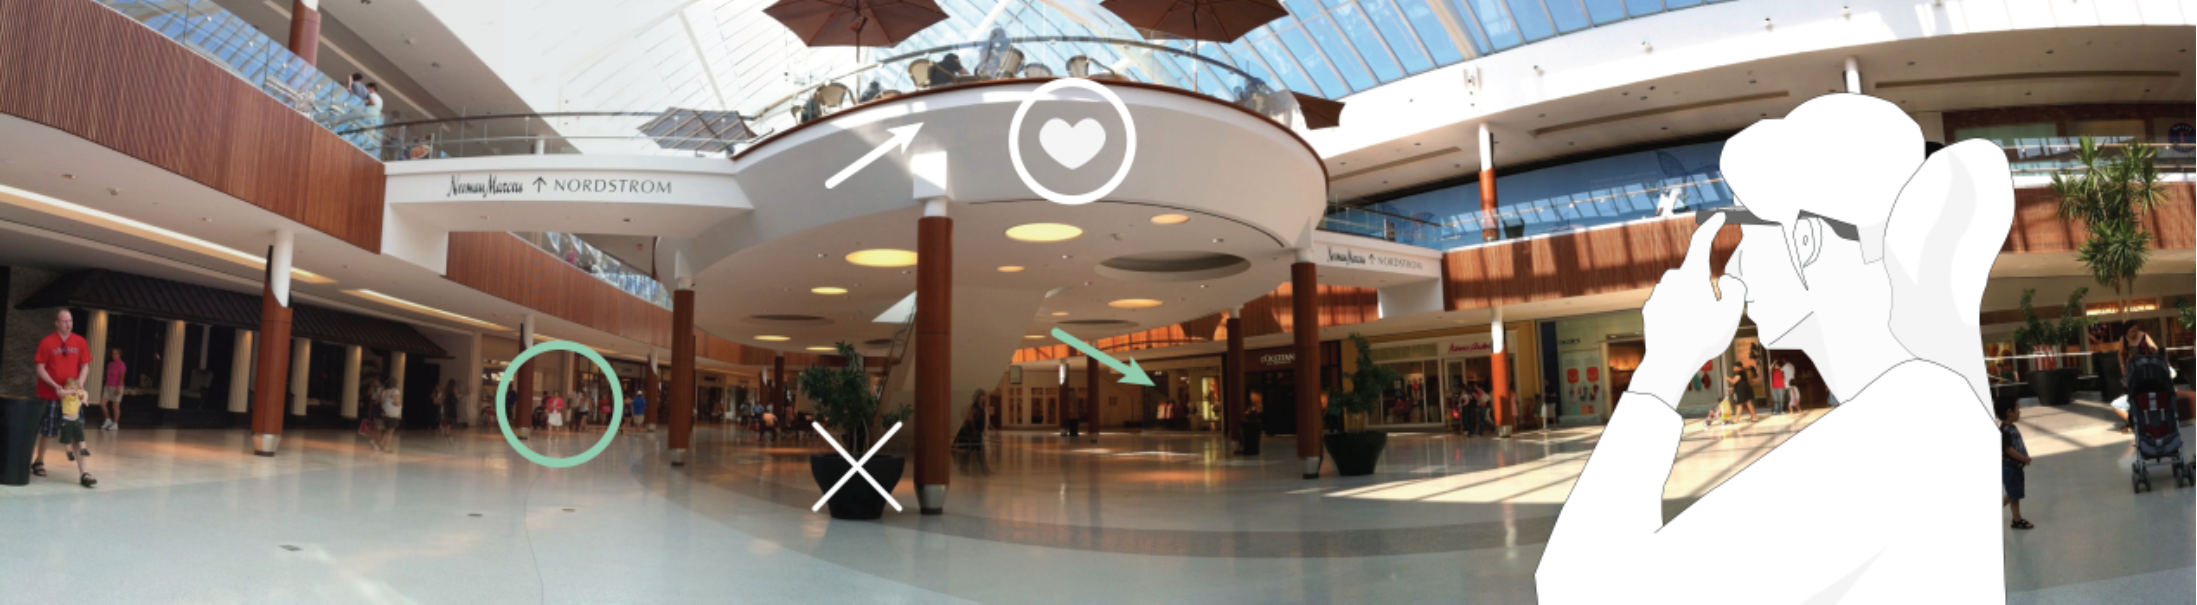
\includegraphics[width=\linewidth]{images/63-pano-ismar14/concept}
    \caption{Social Panoramas using Google Glass}
    \label{fig:ismar14:concept}
\end{figure}

Camera-equipped mobile devices provide a quick way of capturing and sharing experiences and spaces. Wearable computers that combine head-mounted displays (HMDs) and cameras provide new opportunities for collaboration. For example, Google Glass\footnote{http://www.google.com/glass/} has a camera, microphone, and head-worn display.

\subsection{Prototype Development}

In order to explore the concept of social panoramas, a prototype was developed that allowed a user with Google Glass to collaborate with a user on a tablet, both viewing and interacting with the same 360-degree panoramic image via a WiFi network. A Context Compass interface \cite{Suomela2000}  was implemented to provide awareness of the remote user's viewpoint. The prototype was developed using Processing \footnote{http://www.processing.org/} with the Ketai library for sensor support \footnote{https://code.google.com/p/ketai/} and the oscP5 networking library \footnote{http://www.sojamo.de/libraries/oscP5/}. The panorama was mapped onto a cylinder, viewed by the user rotating the tablet or their head with Glass. A within-subject experiment was conducted to compare if interaction possibilities such as drawing and pointing within a panorama can increase Social Presence, or "\textit{the sense of togetherness}" \cite{Basdogan2001}. 

The user interface (Figure \ref{fig:ismar14:pointing-drawing}) of the Glass and the tablet, shows the shared panoramic image in the background. To allow independent view points between the two users, a Context Compass appears as a box on a line on top of the screen. It was designed to give overview information of the real world through head mounted displays. The box moves accordingly to the head orientation on the line, which represents 360 degrees. The remote user is being displayed with a red box - once the rectangles are aligned the users are looking at the same direction. The box moves only linearly.

The two users can interact with each other either using drawing or pointing. For the drawing interaction, the Glass users and tablet users alike could make use of drawing any shapes they like by utilising the touch surface of the tablet or the touchpad on the Glass device. Drawing would be done with one finger. Lifting the finger and touching again would result in a new shape being drawn. The pointing interaction is similar to the drawing interaction, but instead of drawing a continuous line only a pointer in the shape of an arrow would be visible and be used in a sense of pointing to objects or locations. The arrow would always be visible on screen even if not in use.

\subsection{Experiment}

The experiment involved a collaborative task between two subjects in different rooms using Glass and Tablet devices, viewing the same panorama of the Glass user's environment. All subjects used four interaction conditions (Figure \ref{fig:ismar14:pointing-drawing}) that were counterbalanced with the technique of Latin square. The four conditions are:

\begin{itemize}
    \item C1-Audio: both participants used audio to communicate with each other and were able to see the panorama and the Context Compass, but they received no additional virtual cues. 
    \item C2-Pointing: a virtual pointer for each user was added that could be used as a cursor on the panorama.
    \item C3-Drawing: users could make use of the Glass touchpad or the touch surface on the tablet to draw on the panorama. 
    \item C4-Dual: this condition combined the Pointing and Drawing conditions; users were allowed to switch between them.
\end{itemize}{}

C2-Pointing and C3-Drawing was performed by using touchpad input on the side of Google Glass, or touching the Tablet screen. After each trial, subjects filled out a Social Presence questionnaire consisting of eight questions on a seven-point Likert scale taken from Basdogan et al. \cite{Basdogan2001}. Usability was also measured with the System Usability Scale (SUS) \cite{brooke1996sus}.

\begin{figure}
    \centering
    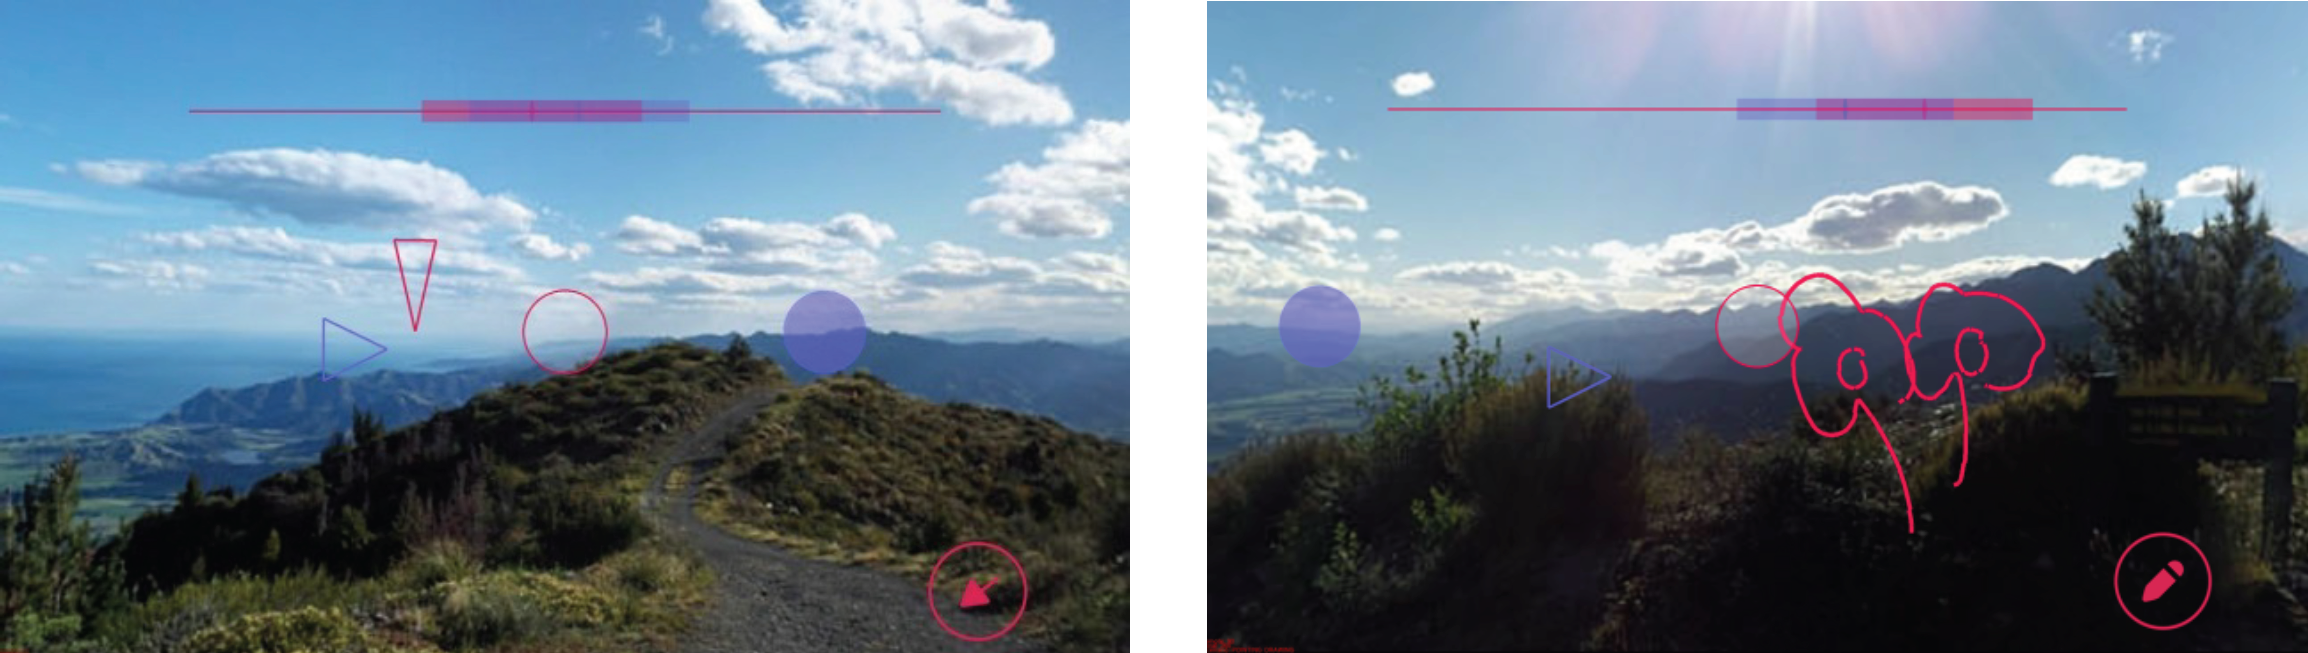
\includegraphics[width=\linewidth]{images/63-pano-ismar14/pointing-drawing}
    \caption{Triangular pointing cursor on the left, and drawing on the right. An icon indicates in which mode the user is.}
    \label{fig:ismar14:pointing-drawing}
\end{figure}

The subjects were given a list of furniture objects printed on a paper to describe to the other user the shape and discuss where to place this furniture item. Both of them could see the name of the object (e.g., "Mirror"), but only one could see the picture attached to it. The subject without the accompanying picture was asked to find a suitable place inside the panorama room (Figure \ref{fig:ismar14:envrionment-setup}), while the other would give a description and confirm or deny if the location was deemed realistic. Once both participants had agreed on a location, they would move on to the next object. They were given a maximum of three minutes. The Glass user was tasked to place objects in the room that they are in under guidance from the tablet person.

\begin{figure}
    \centering
    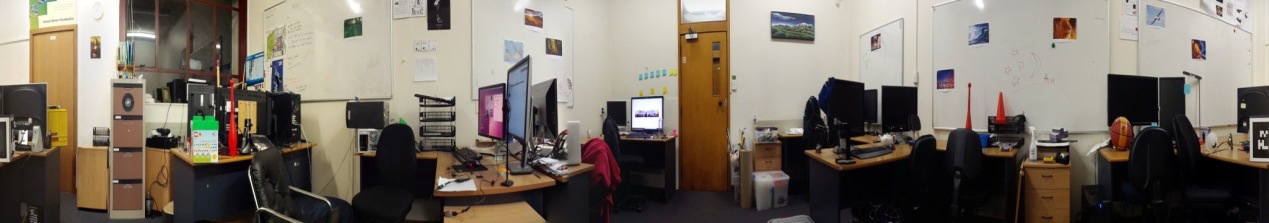
\includegraphics[width=\linewidth]{images/63-pano-ismar14/envrionment-setup}
    \caption{Panorama used for the study. The room represents the room of the Glass user.}
    \label{fig:ismar14:envrionment-setup}
\end{figure}

\subsection{Results}

There were 24 subjects aged between 18 and 45, divided into groups of two. Subjects did not know each other prior to the experiment and collaborated in pairs of their own gender to avoid any biases based on gender. Gender was equally distributed. Social Presence was measured as one single dimension. Figure \ref{fig:ismar14:social-presence} shows the overall Median values for each condition. The Drawing condition on Glass had a significantly lower Social Presence due to limited touch space on the Glass touchpad. 

The results of all eight questions of the Social Presence questionnaire were analysed with a Friedman test, which revealed a significant difference between the conditions for Glass users. ($\chi^2(3)=18.130, p<0.0005$). The significance level was set to p=0.0083 when a Bonferroni correction was applied. The following conditions were significantly different: Drawing-Audio ($Z=-3.794, p<0.0005$) and Drawing-Dual ($Z=-3.103, p=0.002$), resulting in Audio scoring the highest. There was no significant difference for tablet users.

\begin{figure}
    \centering
    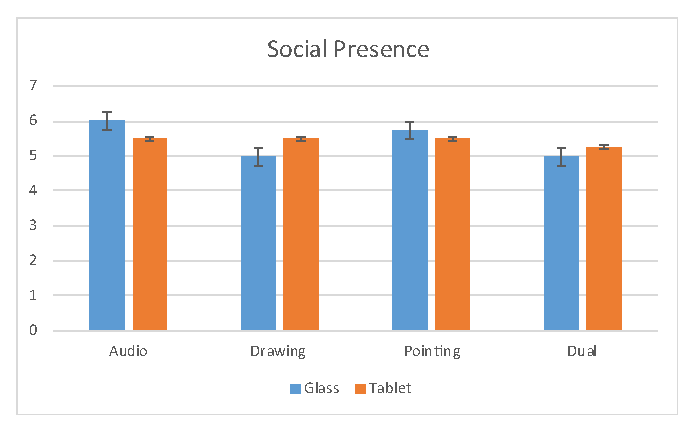
\includegraphics[width=.8\linewidth]{images/63-pano-ismar14/images-02.eps}
    \caption{Average results of social presence between glass and tablet}
    \label{fig:ismar14:social-presence}
\end{figure}

% \begin{table}[ht]
%     % Please add the following required packages to your document preamble:
%     % \usepackage{booktabs}
%     \caption{Median Social Presence values}
%     \centering
%     \begin{tabular}{@{}lllll@{}}
%     \toprule
%     \textbf{}       & \textbf{Audio} & \textbf{Drawing} & \textbf{Pointing} & \textbf{Dual} \\ \midrule
%     \textbf{Glass}  & 6              & 5                & 5.8               & 5             \\
%     \textbf{Tablet} & 5.5            & 5.5              & 5.5               & 5.3           \\ \bottomrule
%     \end{tabular}
%     \label{tbl:ismar14-results}
% \end{table}

The SUS survey (Figure \ref{fig:ismar14:sus}) was used to measure the usability of the interfaces, and both the Glass and tablet conditions were found to have good usability. The tablet Audio scored the highest with an average of $77.1\pm18.9$, which indicates a "good" usability \cite{Bangor2008}. Furthermore, the Drawing and Pointing conditions scored $70.4\pm21.4$ and $74.2\pm21.5$ respectively, also rated "good". However, the Dual condition scored merely $62.9\pm24$, reflecting the observation that users preferred to stay on one interaction tool during the Dual condition.

On Glass, the Audio usability was highest ($75.6\pm10.8$) followed by Pointing ($72.1\pm17.1$). The Dual mode was ranked as unacceptable ($58.1\pm18.6$) together with Drawing ($53.8\pm19.2$), showing the Glass touchpad was perceived as too difficult for drawing. A repeated-measures ANOVA determined that mean SUS scores differed statistically significantly between the conditions ($F(3, 33)=5,625025, P=0.003$) for Glass. There was a significant difference between Audio and the Drawing ($p<0.05$). A number of observations of user behaviour can be made. 
% Drawings were more commonly made to explain shape and dimensions, and pointing gestures were usually used to reference a location or an exact object. 

\begin{figure}
    \centering
    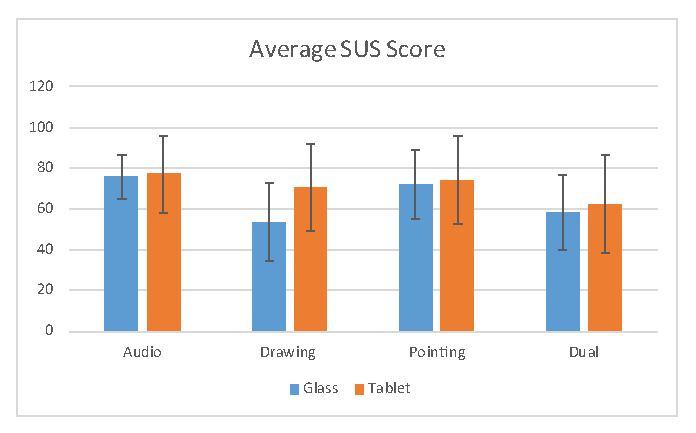
\includegraphics[width=.8\linewidth]{images/63-pano-ismar14/images-01.eps}
    \caption{Average results of SUS between glass and tablet}
    \label{fig:ismar14:sus}
\end{figure}

Tablet users generally preferred drawing to pointing and tried to draw the object shape (Figure \ref{fig:ismar14:tablet-drawing}). Due to difficulties with the touchpad, Glass users ended up using more abstract representations, such as rectangles or circles.

\begin{figure}
    \centering
    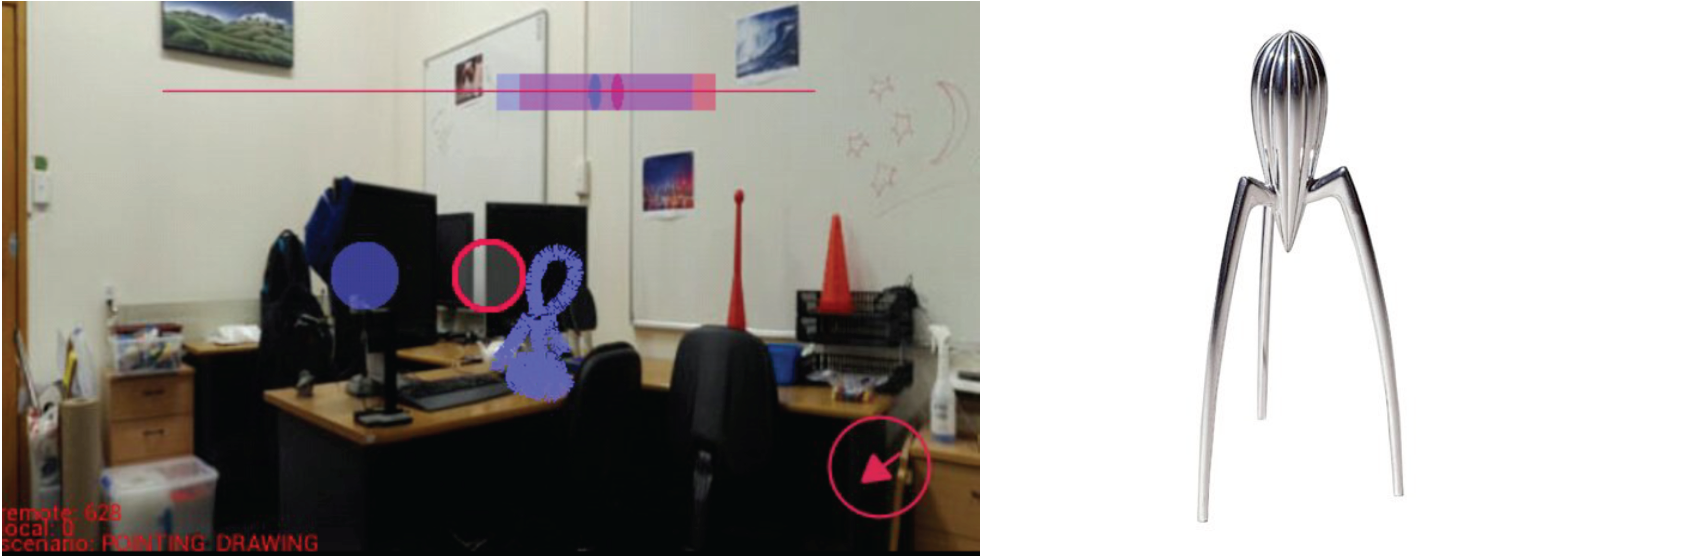
\includegraphics[width=\linewidth]{images/63-pano-ismar14/tablet-drawing}
    \caption{Tablet user attempting to draw an orange juicer}
    \label{fig:ismar14:tablet-drawing}
\end{figure}

\subsection{Observations}

Drawings were more commonly made to explain object shape and dimensions, and pointing gestures were usually used to reference a location or an exact object. Due to limited space of touchpad on Glass, adding drawing and pointing options did not increase social presence.
% The Audio condition was the highest score in social Presence due to a lower level of interactivity between subjects and potential misunderstanding during the conversation when relying on Audio only to communicate. 

Local (Glass) users seemed to be engaged with the remote (Tablet) user by 1) following the orientation cues and being aware of their orientation comparing to the remote user's orientation, 2) being able to annotate (draw and point) on the image to improve their communication. The benefit of sharing panorama is to see the surrounding environment of the remote user, and have mirrored experiences.

This experiment found that adding interaction tools did not increase the Social Presence, compared to the Audio only interface. Users found drawing on the Glass touch pad difficult to use and ranked this as the worst condition for Social Presence, suggesting if a Social Panorama interface is not easy to use it will have a negative impact on Social Presence. 

% The results show that effective shared social experiences can be developed with panorama imagery, but more work still needs to be done. 

\subsection{Conclusions}

This section described the concept of Social Panoramas, using wearable computers, cameras and displays to share spaces in real-time. A prototype was developed on Google Glass and then used to explore the impact of interaction on Social Presence in a user study. 

Results found a difference in Social Presence between the Audio only condition and those that involved drawing interaction on Glass. Similarly, Audio scored the highest on Glass for usability compared to the Drawing and Dual condition. There was a clear preference from users for pointing tools. However, drawing on the Glass touchpad was perceived as difficult. These results show that effective, shared social experiences can be developed with panorama imagery, but more work still needs to be done.
Desipte adding higher fidelity of annotation (drawing or pointing), in this specific platform (Glass), it did not lead to higher social presence. This indicates that it is important to have flexible a platform that supports the interaction method in good usability to gain the ben


% In the future, there are a number of ways that this research could be extended. First, we could explore ways to overcome the drawing problem on Glass, such as using predefined simple geometric shapes such as circles and rectangles that could be observed being drawn during the experiment. Another possibility for future work is to offer a live-stream of the current field of view of the local user, enabling the Mixed Reality view to show a combination of the captured image and live video. These new interface elements will have to be evaluated in a further series of experiments focusing on usability and Social Presence.


\pagebreak
\section{Social Interactions Summary}

The research question of this chapter was \ref{rq:data}: "How can wearable AR displays be used best for interacting with social contacts and shared social data?". This chapter explored different options of representing social interactions in AR including samples of 1) sharing annotations on a panoramic video, 2) sharing 3D annotation using depth cameras, and 3) sharing 360 panoramic images with annotation and awareness cues. These explorations include user studies that measure the social presence, usability and users' feedback/preference. These interactions can be used on the Social AR Continuum to control the interactions between social contacts and shared data based on social proximity. For instance, for a closer relationship, higher fidelity of social interactions (e.g., 3D annotations and drawing) can be enabled, while lower fidelity (e.g., text list annotations and pointing) is for further away from social proximity relationships.

The user study of annotation on live stream video showed that there is a statistically significant difference in the social presence (in particular perceived message understanding and perceived effective understanding) and usability score when a higher level of detail of interaction and annotation is available for participants. The user study of annotation on 3D depth data showed that there is a statistically significant difference in social presence when using 3D annotation. 

The last user study explored different interaction methods, including drawing and pointing as a higher fidelity interaction method aiming to increase social presence. However, the social presence was not increased due to a limitation of the interaction method on the device chosen (Glass) for this experiment.

The following chapter will summarise the conclusions of the entire thesis and highlight a few future directions from this research.

